\documentclass[11pt,twoside]{article}

\usepackage{amsmath}
\usepackage{graphicx,epsfig}
\usepackage{graphicx}
\usepackage{amsmath,amssymb,amsbsy,bm}
%\usepackage[framed]{mcode}

\newlength{\toppush}
\setlength{\toppush}{2\headheight}
\addtolength{\toppush}{\headsep}

\renewcommand{\bottomfraction}{0.95}

\newcommand{\htitle}[3]{\begin{center}
\vspace*{-\toppush}
{\large MASSACHUSETTS INSTITUTE OF TECHNOLOGY}\\
{\small Department of Electrical Engineering and Computer Science}\\
\vspace*{1ex}{\Large #2}\end{center}
\noindent
\newline\parbox{6.5in}
{Fall 2013\hfill Issued : #1 \newline
 Problem Set 2 \hfill Due : #3\newline
%\profs \hfill %Handout #1\vspace*{-.5ex}\newline
%\mbox{}\hrulefill\mbox{}
}}

\newcommand{\mcO}{\mathcal{O}}
\newcommand{\handout}[3]{\thispagestyle{empty}
\pagestyle{myheadings}\htitle{#1}{#2}{#3}}

\setlength{\oddsidemargin}{0pt}
\setlength{\evensidemargin}{0pt}
\setlength{\textwidth}{6.5in}
\setlength{\topmargin}{0in}
\setlength{\textheight}{8.5in}


\newcommand{\pp}[2]{\frac{\partial #1}{\partial #2}}%
\newcommand{\ppp}[2]{\frac{\partial^2 #1}{\partial #2^2}}%
\newcommand{\dd}[2]{\frac{d #1}{d #2}}%
\newcommand{\ddd}[2]{\frac{d^2 #1}{d #2^2}}%
\newcommand{\matend}{\end{array}\right]}
\newcommand{\matc}{\left[\begin{array}{c}}
\newcommand{\matcc}{\left[\begin{array}{cc}}
\newcommand{\bb}{\mathbf{b}}
\newcommand{\bx}{\mathbf{x}}
\newcommand{\bA}{\mathbf{A}}
\newcommand{\DD}[2]{\frac{D #1}{D #2}}%
\newcommand{\Uvec}{\mathbf{U}}
\newcommand{\uvec}{\mathbf{u}}
\newcommand{\tauvec}{\bm{\tau}}
\newcommand{\omegavec}{\bm{\omega}}


\renewcommand{\Re}{\mathrm{Re}}


\begin{document}


\handout{Sept 11, 2013}{6.301 Solid State Circuits}{Sept 18, 2013}
\setlength{\parindent}{0pt}

\newcommand{\solution}{
 \medskip
 {\bf Solution:}
}

\hrulefill

\flushleft
\subsection*{Problem 1: Saturation}
Determine the DC Operating voltage $V_1$ at which $Q_1$ saturates and $V_2$ at which $M_1$ enters the triode regime. \\
Your answer should be in terms of transistor parameters ($I_S$, $V_{CE,sat}$, $\beta_0$, etc).

\begin{center}
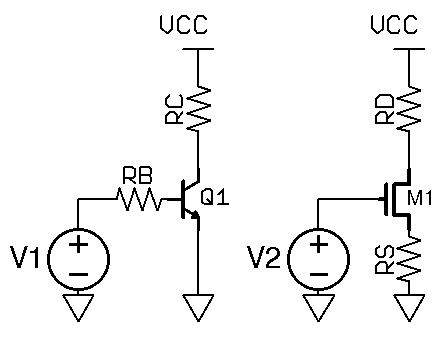
\includegraphics[width=0.35\textwidth]{saturation.png}
\end{center}

\subsection*{Problem 2: Small-signal Parameters}
Calculate the small-signal transistor parameters $g_m$, $r_{\pi}$, and $r_o$ in the following circuit. \\
Assume $V_A = 60v$ and $\beta_0 = 200$.  \\

\begin{center}
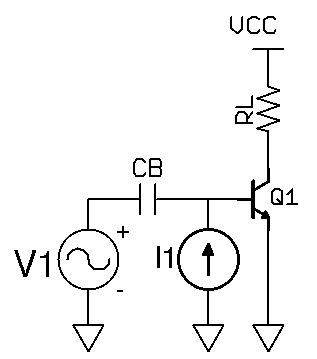
\includegraphics[width=0.25\textwidth]{parameters.png}
\end{center}

\begin{enumerate}
\item[(a)] $I_1 = .5\mu A$
\item[(b)] $I_1 = 50\mu A$
\item[(c)] Draw the small signal model
\item[(d)] How does the bias current $I1$ affect output impedance?
\item[(e)] How does the bias current $I1$ affect input impedance?
\end{enumerate}

\clearpage

\subsection*{Problem 3: Extracting Parameters from Datasheets}
Extract $r_\pi$, $\beta_0$, $r_\mu$, $r_o$, $c_\mu$, and $c_\pi$ from the 2N2222 datasheet posted on stellar.

\vspace{1ex}

\subsection*{Problem 4: Finding $\tau_F$} 
In many cases, datasheets will not provide enough information to extract every transistor parameter.  
Using the 2N3866 datasheet posted on stellar, determine an upper bound on $\tau_F$.  Briefly explain all assumptions that you make and define $\tau_F$ and $f_T$.


\clearpage
\end{document}
